\documentclass[11pt]{report}
\usepackage{array}
\usepackage{makecell}
\usepackage{float}
\usepackage{graphicx}
\usepackage{color,colortbl}
\usepackage{tikz}
\usepackage{pgf}
\usepackage{caption}
\usepackage{subcaption}
\usepackage{pgfplots}
\usepackage{multirow}
\usepackage{amsmath}
\usetikzlibrary{spy,calc}
\usepackage{cite}
\tikzset{boximg/.style={remember picture,red,thick,draw,inner sep=0pt,outer sep=0pt}}
\usepackage{hyperref}
\hypersetup{
    colorlinks=true, %set true for colored links
    linktoc=all,     %set to all if  both sections and subsections linked
    linkcolor=blue,
urlcolor=cyan,  %choose some color 
}

\pagenumbering{roman}
\newcommand{\mychapter}[2]{\setcounter{chapter}{#1}
\setcounter{section}{1}
\chapter*{#2}
\addcontentsline{toc}{chapter}{#2}}
\begin{document}

\title{Software Project Proposal}
\author{Nishat Tasnim - 1305066\\\& Afroza Nowshin - 1305100\\Group no. - 3}
\date{\today}
\maketitle
\newpage
\tableofcontents{}
\listoffigures
\listoftables

\pagenumbering{arabic}
\setcounter{page}{4}
\mychapter{1}{Our Project Proposal}
\paragraph{•}For our CSE-324, that is, Software Development Sessional project, we have chosen to create a web-based application that will assist people in mastering Bangla and/or English language. We are planning to design the software in such a way that both the indigenous and foreign user can easily and effectively learn the languages, without any difficulty. In this pre-project documentation, we have mentioned the motivation of our proposal, which also defines the scope of our project. Then the problems that our project tend to overcome are mentioned. The features of our project are mentioned also. A realistic time-line is also attached which reflects the schedule of the project development. In the end, the snapshots of our tentative Graphical User Interface is attached.
\mychapter{2}{Functionalities}
\section*{Modules}
\paragraph{•}Our software is a single server(admin) and multiple clients system. As per standard software design, we will follow the MVC design pattern in our software. For convenience, we have divided our software into three different modules, each has its own functionalities. They are described in the following:\\
\begin{enumerate}
\item \textbf{Admin Module:} This module is intended for the admin. An admin can add\textbackslash modify a course, add new features for the end users. The admin also has the power of adding\textbackslash deleting\textbackslash updating databases in the back- end.
\item \textbf{Client\textbackslash User Module:} This module represents the front end of our software. Using this module, any user(s) can search for courses. If he is a new user, and want to enrol for any of our course, he will be prompted with a message to register and create an account in our software. Existing user can just log into our system. The databases of new and existing users, groups and courses will all be handled by the admin module.
\item \textbf{Courses Module:} In this module, our courses can be seen, provided by the admin. 
\end{enumerate}
\section*{Parameterization}
\paragraph{•}We will create and develop our software which will serve as a standalone tool for learning English and Bangla. In future, we will use our software to provide courses on French, German, Chinese, Japanese, Spanish, Korean etc. This means that we can parameterize our software to provide courses other than English and Bangla.\\
\section*{Insight generating features}
??????????
\mychapter{3}{Motivation and Why will people use it}
\section*{Motivation}
\begin{itemize}
\item \href{http://www.bbc.com/future/story/20160811-the-amazing-benefits-of-being-bilingual}{Various scientific researches} show that learning a new language in addition to mother tongue helps to sharpen one's recalling power. 
\item Knowing another language besides mother tongue always comes in handy, especially if one goes to a foreign land.
\item Learning a new thing is always fun, and this is equally true for a language.
\end{itemize}
\section*{What we will offer?}
\paragraph{•}To learn a language, one has to enrol to a course, and physically attend each class, to gain an acknowledgement and a certificate for completing the course. Now, the certificate may appear to be lucrative, but there are times when a person cannot attend class. Also, this language courses appear to be quite extravagant. Another issue is that, the teaching staff are not liable to teach the students enrolled to their courses effectively. Whether the student does good or completes the entire language course with a mediocre grade is not the teacher's concern. As a matter of fact, in a classroom full of students coming from all walks of life, it is quite natural that a teacher may not be able to give individual attention to each student. Therefore, even if a person spends a lot of his valuable time and money, he may not learn the foreign language entirely and effectively.
\paragraph{•}With our software, we are ensuring that:\\
\begin{enumerate}
\item Our application is free.
\item User will simply create an account in our application using his email address
\item One can learn \textcolor{blue}{anywhere} and \textcolor{blue}{any time}. No need to be present in a classroom physically.
\item Our application offers a very user-friendly experience.
\item We will offer a number of techniques proven from scientific researches to remember a new word.
\item Audio feature to learn the pronunciation of each word. 
\item Users can create different technique suitable for him and also for others, for example, create `Meme', attach similar enunciating word from his mother tongue.
\item User will be able to customize the application by changing the keyboard shortcut according to his choice.
\item Learning is effective when a particular topic is learnt through group study. In our application, a user can form group with the similar users.
\end{enumerate}
\mychapter{4}{Inspiration from Existing Works}
\paragraph{•}There are a number of applications that are meant to be used in desktop computer or mobile phone. The names are given below:
\begin{itemize}
\item Memrise
\item Duolingo
\item Busuu
\item Lingvist
\item Babbel
\end{itemize}
All of the applications are popular. Among them, in \textcolor{green}{Babbel} and \textcolor{green}{Duolingo}, a user has to buy the whole language course. The rest of the applications are free. All these applications offer a wide variety of languages. \textcolor{green}{Memrise}, although, is not entirely a language learning application. It offers courses on different topics also. None of these applications do not offer course on Bangla language. For our software, we planned to emulate some of the salient features of `Memrise', and our application will assist to learn Bangla as well.
\mychapter{5}{Realistic time line that we will follow}
\paragraph{}As this term is 14 weeks long as usual, we have to complete a full working web based application within this time. A tentative time line mapped to our line of work is given here:~\ref{tab:time}
\begin{table}[!h]
\centering
\caption{Realistic time line table}
\label{tab:time}
\begin{tabular}{|p{2cm}|p{6cm}|}
\hline
\textbf{\thead{Week No.}} &\textbf{\thead{Target}}\\
\hline
5 & Creating GUI, setting up all necessary tools, database and framework and learning the use of Spring MVC framework\\
\hline
6,7 & Creating database for users and admin\\
\hline
Midterm break & Creating database for courses and connecting with the front end\\
\hline
8,9 & Adding audio features\\
\hline
10,11 & Adding group study features\\
\hline
12 & Adding images to individual courses\\
\hline
13 & Adding points, bonus and rank system\\
\hline
14 & Final project submission\\
\hline
\end{tabular}
\end{table}
\mychapter{6}{Tools \& Technologies that we will use}
\paragraph{•}The tools that we are planning to use in our project is given in the table:~\ref{tab:tool}. 
\begin{table}[!h]
\centering
\caption{Tools that will be used}
\label{tab:tool}
\begin{tabular}{|l|p{4cm}|}
\hline
\textbf{\thead{Tool} }& \textbf{Name}\\
\hline
Programming Language & Java\\
\hline
IDE & \thead{Intellij IDEA\\Ultimate version,\\Netbeans platform\\SDK(Java EE),\\Eclipse}\\
\hline
Framework & Spring MVC\\
\hline
Database & Oracle\\
\hline
Styling & HTML, CSS\\
\hline
\end{tabular}
\end{table}
\paragraph{•}This is a basic list, and not complete. Throughout the project this list will expand.
\mychapter{7}{Snapshots of Graphical User Interfaces}
\paragraph{•}Following are some sample images of the graphical user interfaces ~\ref{fig:sign}, ~\ref{fig:pro}, ~\ref{fig:cou}, ~\ref{fig:home}, ~\ref{fig:grp}. These are mere samples, and may change as required for the project.
\begin{figure}[!h]
\centering
\includegraphics[width=.80\textwidth]{sample1_sign.png}
\caption{Sign Up Form}
\label{fig:sign}
\end{figure}
\begin{figure}[!h]
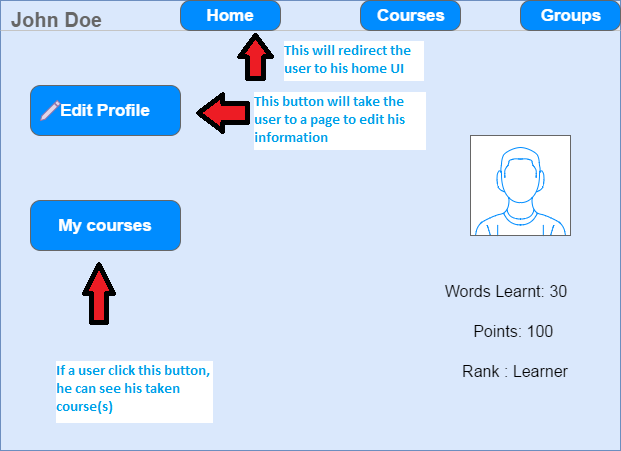
\includegraphics[width=1.0\textwidth]{sample2_profile.png}
\caption{User Profile Form}
\label{fig:pro}
\end{figure}
\begin{figure}[!h]
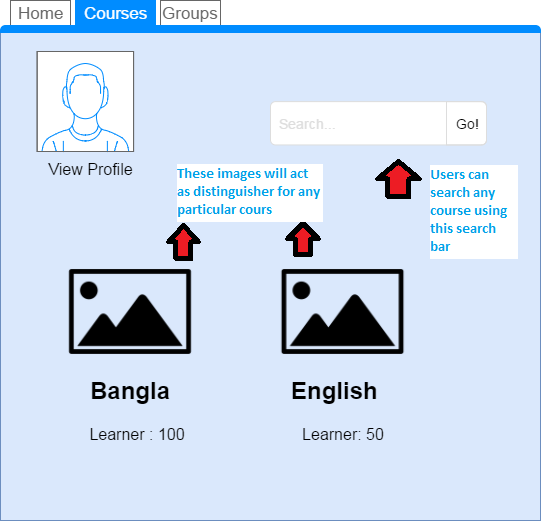
\includegraphics[width=1.0\textwidth]{sample3_courses.png}
\caption{User Course Form}
\label{fig:cou}
\end{figure}
\begin{figure}[!h]
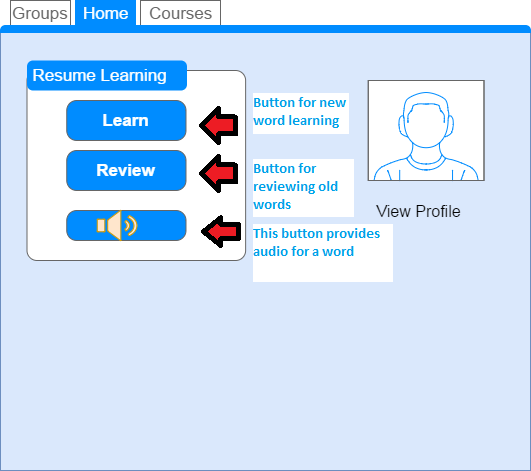
\includegraphics[width=1.0\textwidth]{sample4_home.png}
\caption{User Home Form}
\label{fig:home}
\end{figure}
\begin{figure}[!h]
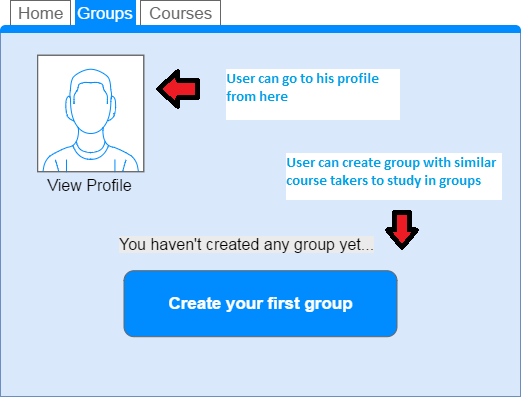
\includegraphics[width=1.0\textwidth]{sample5_groups.png}
\caption{User Group Form}
\label{fig:grp}
\end{figure}
\mychapter{8}{List of external links}
\begin{enumerate}
\item \url{https://docs.spring.io/spring/docs/current/spring-framework-reference/html/mvc.html}
\item \url{https://www.memrise.com/}\\
\item \url{https://www.duolingo.com/}\\
\item \url{https://www.busuu.com/}\\
\item \url{https://lingvist.com/}\\
\item \url{https://www.babbel.com/}\\
\item \url{http://www.bbc.com/future/story/20160811-the-amazing-benefits-of-being-bilingual}\\
\item \url{https://netbeans.org/}\\
\item \url{https://www.jetbrains.com/idea/}\\
\item \url{https://eclipse.org/}\\
\item \url{https://www.oracle.com/}\\
\end{enumerate}
\end{document}